\documentclass[10 pt]{article}
\usepackage{tikz}
\usetikzlibrary{arrows}
\usepackage[margin=0.5 in]{geometry}
\usepackage[utf8]{inputenc}
\usepackage{tabu}
\usepackage{color}
\usepackage{xcolor}
\usepackage{listings}
\usepackage{enumitem}
\usepackage{multicol}
\setlength{\columnsep}{1cm} 
\title{\textbf {Estructuras de Datos 1 - ST0245\\Segundo Parcial}}
\author{Nombre ..............................\\
		Departamento de Informática y Sistemas\\
		Universidad EAFIT\\}
\date{Octubre 23 de 2018}
\begin{document}
\lstdefinestyle{customc}{
	language=Java, 
	numbers=left, 
	showspaces=false,
    showstringspaces=false, 
    tabsize=2, 
    breaklines=true,
    xleftmargin=5.0ex,
}
\lstset{escapechar=@,style=customc, numbers=left, stepnumber = 1} 
\maketitle
\begin{multicols}{2}
Para propósitos de este parcial, se considerará esta implementación de un árbol binario y sus estos recorridos.
{\footnotesize
\begin{lstlisting}
//Arbol binario
class BNode{
  BNode izq;
  BNode der;
  int val;
}

//Recorridos
void preorden(BNode nodo){
  if(nodo != null){
    System.out.println(nodo.val);
    preorden(nodo.izq);
    preorden(nodo.der);  
  }
}
void posorden(BNode nodo){
  if(nodo != null){
    posorden(nodo.izq);
    posorden(nodo.der);
    System.out.println(nodo.val);  
  }
}
void inorden(BNode nodo){
  if(nodo != null){
    inorden(nodo.izq);
    System.out.println(nodo.val);
    inorden(nodo.der);  
  }
}
\end{lstlisting}
}
\section{Pilas y Colas 30\%}
Polka desea implementar una cola de una manera muy especial: Él ya tiene implementada una pila, pero no quiere implementar una cola desde el principio, entonces él  ha decido usar la pila que ya tiene implementada para implementar la cola. Él quedará conforme si implementa las dos funciones principales de la cola: \texttt{offer(e)} (añade el elemento $e$ al inicio de la cola), \texttt{poll()} (extrae y elimina el primer elemento que entró a la cola). Él ya implementó \texttt{offer(e)}, pero  no ha podido con \texttt{poll()}, entonces él quiere que tú lo implementes. Las variables $s1,s2$ son dos pilas que se inicializan en el constructor de la clase \texttt{Cola}.

{\small
\textbf{Nota: } En una pila, la función \texttt{pop()} retorna y extrae el elemento en el tope de la pila, y la funcion \texttt{push(x)} añade el elemento $x$ al tope de la pila.

\textbf{Nota 2:} En la vida real no se implementa una cola con pilas porque no es eficiente.
}
\begin{lstlisting}
class Cola{
  Stack<Integer> s1, s2;
  Cola(){
    s1 = new LinkedList<>();
    s2 = new LinkedList<>();
  }
  void offer(int e){
    s1.push(e);
  }
  int poll(){
  	//Completa por favor
  	if(s2.isEmpty()){
  	  while(______________)
  	     s2.push(___________);		
  	  }
  	}
  	return ___________; 
  }
}
\end{lstlisting}
\begin{enumerate}[label=(\roman*)]
% Respuesta: !s1.isEmpty()
\item (10\%) Completa la línea 13 ................
% Respuesta: s1.pop()
\item (10\%) Completa la línea 14 ................
% Respuesta: s2.pop()
\item (10\%) Completa la línea 17 ...............
\end{enumerate}
\section{Árboles 30\%}
\textbf{Nota: }El sub-índice $D$ indica que el nodo es un hijo derecho con respecto a su padre. El sub-índice $I$ indica que es un hijo izquierdo con respecto a su padre. 
\begin{center}
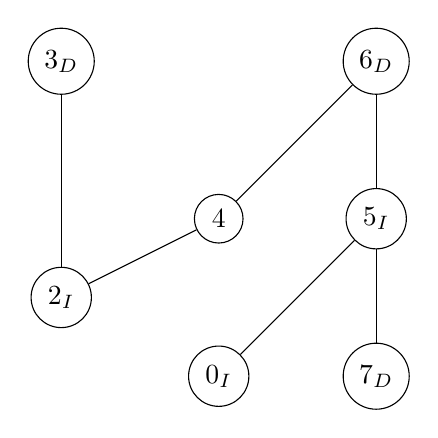
\begin{tikzpicture}

\tikzset{vertex/.style = {shape=circle,draw,minimum size=1.2em}}
\tikzset{edge/.style = {-,> = latex'}}
\node[vertex] (4) at (0,0)  {4};
\node[vertex] (2) at (-2,-1)  {$2_I$};
\node[vertex] (5) at (2, 0) {$5_I$};
\node[vertex] (3) at (-2, 2) {$3_D$};
\node[vertex] (0) at (0, -2) {$0_I$};
\node[vertex] (7) at (2, -2) {$7_D$};
\node[vertex] (6) at (2, 2) {$6_D$};

%edges
\draw[edge] (4) to (2);
\draw[edge] (6) to (5);
\draw[edge] (5) to (0);
\draw[edge] (4) to (6);
\draw[edge] (5) to (7);
\draw[edge] (2) to (3);
\end{tikzpicture}
\end{center}
\begin{enumerate}[label=\alph*]
\item (10\%) ¿Cuál es la salida del recorrido en \textit{in-orden} del árbol anterior, tomando el nodo $4$ como el nodo raíz? 
\begin{enumerate}[label=(\roman*)]
% Respuesta: 2, 3, 4, 0, 5, 7, 6
\item 3, 2, 0, 7, 5, 6, 4
\item 2, 3, 4, 0, 5, 7, 6 
\item 4, 2, 3, 6, 0, 5, 7
\item 4, 7, 3, 6, 2, 0, 5   
\end{enumerate}
\item (10\%) Asuma que el nodo $4$ es la raíz del árbol binario anterior. Asuma que la salida del recorrido \textit{pre-orden} es $\{a_1,a_2,a_3,...,a_n\}$ y la salida del recorrido \textit{in-orden} es $\{b_1,b_2,b_3,...,b_n\}$. ¿Cuál es el primer valor de $i$ para el cual $a_i=b_i$?  Note que la $i$ empieza en 1.
\begin{enumerate}[label=(\roman*)]
%Respuesta: 5
\item 5
\item 4
\item 3
\item 2  
\end{enumerate}
Por ejemplo, asuma que las salidas son $a = \{4, 6, 5, 0, 7, 2, 3\}$ y $b = \{6, 4, 7, 0, 5, 2, 3\}$. La respuesta sería 4 porque $a_4 = b_4 = 0$ e $i=4$ es el primer valor para el que $a_i=b_i$. 

\item (10\%) ¿Es un \textbf{\textit{árbol binario de búsqueda}} el árbol anterior?
\begin{enumerate}[label=(\roman*)]
% Respuesta: Sí
\item Sí
\item No
\end{enumerate}
\end{enumerate}
\section{Listas 30\%}
El método \texttt{add(x)} agrega el elemento $x$ al fin de la lista. El método \texttt{get(i)} retorna el valor en la posición $i$ de la lista. El metodo \texttt{remove(i)} elimina el elemento en la posición $i$ en la lista. Considere el siguiente método y asuma que el método se llama con una lista vacía $l$. El operador \% es el residuo de la división entera de dos enteros.
\begin{lstlisting}
int metodo
(LinkedList<Integer> l,int a,int b){
  int i=0;
  for(int j=a;j<=b;j++){
    int s=j;
    while(s > 0){
      l.add(s%10);
      i=(i+1)%l.size(); 
      s=s/10; //division entera
    }
  }
  return l.get(i);
}
\end{lstlisting}
\begin{enumerate}[label=\alph*]
\item (10\%) ¿Cuál es la complejidad asintótica, \textbf{en el peor de los casos}, del algoritmo anterior? Asuma que $a-b<0$.
\begin{enumerate}[label=(\roman*)]
%Respuesta: O(|b-a|*log10 b)
\item $O(|b-a|\times \log_{10} b)$
\item $O(|b-a|)$
\item $O(|b-a|\times \log_2 |b-a|)$
\item $O(|b-a|^2)$
\end{enumerate}
\item (10\%) ¿Qué imprime el algoritmo anterior cuando $a=2,b=7$? Como un ejemplo, para $a=2, b=5$ la respuesta es $5$. 
\begin{enumerate}[label=(\roman*)]
%Respuesta: 7
\item 3
\item 7
\item 4
\item 5
\end{enumerate}
\item (10\%) ¿Cuál es la complejidad asintótica, \textbf{en el peor de los casos}, de \texttt{remove(i)} en una lista enlazada?
\begin{enumerate}[label=(\roman*)]
%Respuesta: O(n)
\item $O(\log n)$
\item $O(n)$
\item $O(1)$
\item $O(n^2)$
\end{enumerate}
\end{enumerate}
\section{Grafos 10\%}
Un grafo con matrices de adyacencia se puede definir como \texttt{int [][] grafoAM}.
El método para obtener los sucesores de cierto vértice (\texttt{vertex}) tiene que
recorrer la matriz buscando los vértices a los que se puede llegar a partir de \texttt{vertex}.
Las filas representan el origen y las columnas el destino. En la matriz se guarda el peso que hay para llegar de un origen a un
destino. Si no hay conexión entre un origen y un destino, se coloca el valor $0$ en esa casilla.
Juanito hizo el siguiente código, ayúdalo a completarlo.

\begin{lstlisting}
class Graph {
  private int [][] grafoAM;
  public ArrayList<Integer> getSuccessors(int vertex) {
    ArrayList<Integer> sucesores = new ArrayList<Integer>();
    for(int i = 0;i < size;i++){           
      if(......){
           sucesores.add(i);
      }
    }
    return sucesores;
  }
}
\end{lstlisting}
%grafoAM[vertex][i] != 0
\begin{enumerate}[label=\alph*]
\item (10\%) Complete la línea 6 ......................
\end{enumerate}
% Considera el siguiente grafo:
% \\
% \begin{center}
% \begin{tikzpicture}

% \tikzset{vertex/.style = {shape=circle,draw,minimum size=1.2em}}
% \tikzset{edge/.style = {-,> = latex'}}
% \node[vertex] (4) at (0,0)  {4};
% \node[vertex] (2) at (2,2)  {2};
% \node[vertex] (0) at (2,-2)  {0};
% \node[vertex] (1) at (-2, -2) {1};
% \node[vertex] (5) at (0, -4) {5};
% \node[vertex] (3) at (0, 4) {3};
% %edges
% \draw[edge] (4) to (2);
% \draw[edge] (4) to (0);
% \draw[edge] (1) to (4);
% \draw[edge] (1) to (5);
% \end{tikzpicture}
% \end{center}

% \begin{enumerate}[label=\alph*]
% \item (10\%) Completa su representación utilizando listas de adyacencia:
% \\
% %4->0->2->1
% $4 \rightarrow 0 \rightarrow 2 \rightarrow 1$
% \\
% %2->4
% $2 \rightarrow$
% \\
% %0->4
% $0 \rightarrow$
% \\
% %1->4->5
% $1 \rightarrow$
% \\
% %5->1
% $5 \rightarrow$
% \\
% %3
% $3 \rightarrow$
% \end{enumerate}
% \textbf{Pista:} La pregunta NO es calcular la clausura transitiva del grafo, sino la
% lista de las adyacencias, es decir, la lista de los vecinos.
\end{multicols}

\end{document}